\chapter{Lý thuyết phiếm hàm mật độ (DFT)}
\label{ch:dft}

Các chương trước đều làm việc với hàm sóng, một hàm $3N$ chiều, và đều phải trả giá trước bức tường hàm mũ. DFT đặt một câu hỏi táo bạo: \emph{có thể bỏ hẳn hàm sóng, chỉ dùng mật độ electron, một hàm 3 chiều, không?} Câu trả lời ``có, về nguyên tắc'' đã mang về giải Nobel Hóa học 1998 cho Walter Kohn. Ngày nay DFT là phương pháp được dùng nhiều nhất trong hóa học và khoa học vật liệu.

\section{Ý tưởng: bản đồ mật độ thay cho danh sách tọa độ}

\begin{eli5}[bản đồ nhiệt của sân vận động]
Muốn biết một sân vận động đông người ``cư xử'' ra sao, thay vì theo dõi tọa độ của từng người, ta chỉ cần một \emph{bản đồ nhiệt} cho biết mỗi mét vuông có bao nhiêu người. Với 50\,000 người, danh sách tọa độ có 100\,000 con số và tăng theo số người; bản đồ nhiệt thì kích thước cố định. DFT khẳng định rằng với electron ở trạng thái cơ bản, ``bản đồ mật độ'' này, nếu đọc đúng cách, chứa \emph{toàn bộ} thông tin.
\end{eli5}

\begin{congthuc}[mật độ electron]
\[
n(\vr)=N\sum_{\text{spin}}\int|\Psi(\vr,\vx_2,\ldots,\vx_N)|^2\,d\vx_2\cdots d\vx_N ,\qquad \int n(\vr)\,d\vr=N .
\]
$n(\vr)\,d\vr$ là số electron trung bình trong thể tích nhỏ $d\vr$ quanh điểm $\vr$. Dù $N$ lớn bao nhiêu, $n$ chỉ phụ thuộc 3 biến. Đây là đại lượng đo được bằng nhiễu xạ tia X.
\end{congthuc}

\subsection{Phiếm hàm là gì?}
Một \textbf{hàm} nhận một \emph{số} và trả về một số: $f(x)=x^2$. Một \textbf{phiếm hàm} \en{functional} nhận cả một \emph{hàm} và trả về một số; ta viết với ngoặc vuông $F[n]$. Ví dụ đời thường: ``lượng sơn cần dùng'' là phiếm hàm của ``hàm độ dày lớp sơn trên tường''. Ví dụ trong DFT:
\begin{itemize}
\item Số electron: $N[n]=\int n(\vr)\,d\vr$.
\item Năng lượng hút hạt nhân: $V_{\rm ext}[n]=\int\big(-\tfrac{Z}{r}\big)\,n(\vr)\,d\vr$.
\item Năng lượng Hartree, tức lực đẩy cổ điển của ``đám mây'' điện tích với chính nó: $J[n]=\tfrac12\iint\dfrac{n(\vr)\,n(\vr')}{|\vr-\vr'|}\,d\vr\,d\vr'$.
\end{itemize}

\subsection{Tiền thân: mô hình Thomas--Fermi (1927)}
Thomas và Fermi coi electron trong mỗi ô nhỏ của nguyên tử như một ``khí electron đồng nhất'', và viết động năng là $C_F\int n^{5/3}d\vr$. Mô hình cho năng lượng nguyên tử $E_{\rm TF}=-0.7687\,Z^{7/3}\Ha$ \cite{ParrGhosh1986}. Với Li, con số này là $-9.98\Ha$, sai tới 33\%. Tệ hơn, mô hình không có cấu trúc lớp vỏ, và Teller (1962) chứng minh rằng trong mô hình Thomas--Fermi \emph{không phân tử nào bền}: năng lượng phân tử luôn cao hơn tổng năng lượng các nguyên tử \cite{Teller1962}. Một lý thuyết hóa học mà không có liên kết hóa học! Phải chờ gần 40 năm để ý tưởng ``dùng mật độ'' có nền móng vững chắc.

\section{Định lý Hohenberg--Kohn (1964)}

\begin{eli5}[cuốn sách công thức không ai tìm thấy]
Hãy tưởng tượng một ``máy dò'' chỉ nhìn được bản đồ mật độ electron. Định lý Hohenberg--Kohn nói: chỉ từ bản đồ đó, máy suy ra được \emph{nguyên tử nào} đang ở đâu, và do đó suy ra được \emph{mọi thứ khác}. Có một ``công thức'' biến mật độ thành năng lượng. Nhưng định lý chỉ nói công thức đó \emph{tồn tại}, không đưa cho ta công thức. Giống như biết chắc có một cuốn sách công thức nấu ăn hoàn hảo, nhưng chưa ai tìm thấy nó.
\end{eli5}

\begin{congthuc}[hai định lý Hohenberg--Kohn]
Hamiltonian của mọi nguyên tử, phân tử có dạng $\Hhat=\hat T+\hat V_{ee}+\sum_iv(\vr_i)$. Hai số hạng đầu (động năng, đẩy nhau) giống hệt nhau cho mọi hệ; chỉ có thế ngoài $v(\vr)$ (với nguyên tử là $-Z/r$) và số electron $N$ là khác.

\textbf{Định lý 1.} Mật độ cơ bản $n_0(\vr)$ xác định duy nhất thế ngoài $v(\vr)$ (sai khác một hằng số). Do đó $n_0$ xác định $\Hhat$, và mọi tính chất của hệ.

\emph{Chứng minh phản chứng.} Giả sử hai thế $v\neq v'$ cho cùng mật độ $n$, với hai hàm sóng cơ bản $\Psi\neq\Psi'$. Áp dụng nguyên lý biến phân hai lần:
\[
E_0<\langle\Psi'|\Hhat|\Psi'\rangle=E_0'+\!\int(v-v')\,n\,d\vr,\qquad
E_0'<\langle\Psi|\Hhat'|\Psi\rangle=E_0+\!\int(v'-v)\,n\,d\vr .
\]
Cộng hai vế: $E_0+E_0'<E_0+E_0'$, vô lý. Vậy không thể có hai thế khác nhau cho cùng một mật độ.

\textbf{Định lý 2.} Tồn tại một phiếm hàm \emph{phổ quát} $F[n]$ (giống nhau cho mọi nguyên tử, phân tử) sao cho
\[
E_v[n]=F[n]+\int v(\vr)\,n(\vr)\,d\vr\;\ge\;E_0,
\]
dấu bằng khi $n$ là mật độ cơ bản đúng. Tức là có một nguyên lý biến phân cho mật độ \cite{HohenbergKohn1964}.
\end{congthuc}

Điều định lý \emph{không} nói: dạng cụ thể của $F[n]$. Mọi khó khăn của bài toán nhiều electron giờ được dồn vào việc tìm $F[n]$.

\section{Lược đồ Kohn--Sham (1965)}

Thử viết $F[n]$ trực tiếp bằng mật độ (như Thomas--Fermi) thì phần động năng sai rất nặng. Kohn và Sham nghĩ ra một mẹo thông minh \cite{KohnSham1965}.

\begin{eli5}[diễn viên đóng thế]
Thay vì giải bài toán các electron ``cãi nhau'' với nhau, Kohn và Sham thuê một đoàn ``diễn viên đóng thế'' \emph{không hề tương tác}, đặt họ trên một ``sân khấu'' (một thế hiệu dụng) được thiết kế khéo tới mức ảnh chụp đám đông diễn viên (mật độ) giống hệt ảnh chụp đám electron thật. Diễn viên không tương tác thì dễ mô tả: mỗi người chiếm một orbital, và động năng của họ tính chính xác được. Mọi phần khó, tức là việc electron né nhau, được gói vào \emph{một} số hạng duy nhất: năng lượng trao đổi--tương quan $E_{xc}$.
\end{eli5}

\begin{congthuc}[phương trình Kohn--Sham]
Năng lượng toàn phần được tách thành
\[
E[n]=\underbrace{T_s[n]}_{\text{động năng hệ không tương tác}}+\underbrace{\int v_{\rm ext}\,n\,d\vr}_{\text{hút hạt nhân}}+\underbrace{J[n]}_{\text{Hartree}}+\underbrace{E_{xc}[n]}_{\text{mọi thứ còn lại}} .
\]
Các orbital Kohn--Sham thỏa phương trình kiểu Schrödinger một electron:
\[
\Big[-\tfrac12\nabla^2+v_{\rm ext}(\vr)+v_H(\vr)+v_{xc}(\vr)\Big]\varphi_i(\vr)=\varepsilon_i\varphi_i(\vr),\qquad n(\vr)=\sum_{i}^{\text{chiếm}}|\varphi_i(\vr)|^2,
\]
với thế Hartree $v_H(\vr)=\int\frac{n(\vr')}{|\vr-\vr'|}d\vr'$ và thế trao đổi--tương quan $v_{xc}(\vr)=\delta E_{xc}/\delta n(\vr)$ (đạo hàm phiếm hàm: ``thêm một chút mật độ tại $\vr$ thì $E_{xc}$ đổi bao nhiêu'').
\begin{itemize}
\item $E_{xc}=(T-T_s)+(V_{ee}-J)$: gồm phần động năng tương quan, và phần tương tác electron ``phi cổ điển'' (trao đổi, tương quan, và việc sửa lỗi electron tự đẩy chính mình chứa trong $J$).
\item Vì thế phụ thuộc mật độ, mật độ phụ thuộc thế, nên phải giải lặp tới tự hợp, đúng như Hartree--Fock.
\item Với Li (phân cực spin): orbital 1s$\uparrow$, 2s$\uparrow$, 1s$\downarrow$; mỗi spin có thế $v_{xc}^\sigma$ riêng.
\end{itemize}
\end{congthuc}

Nếu biết $E_{xc}$ chính xác, Kohn--Sham cho năng lượng và mật độ \emph{chính xác}. Với Li, $E_{xc}\approx-1.83\Ha$ trên tổng $-7.48\Ha$; riêng phần tương quan chỉ $-0.045\Ha$. Toàn bộ nghệ thuật của DFT hiện đại là xấp xỉ $E_{xc}$.

\begin{hieulam}[orbital Kohn--Sham là orbital ``thật'']
Định thức dựng từ orbital Kohn--Sham \emph{không} phải hàm sóng thật của hệ; orbital KS là công cụ phụ trợ để tính đúng mật độ. Chỉ có một ngoại lệ quan trọng: với phiếm hàm chính xác, năng lượng orbital cao nhất bằng đúng trừ năng lượng ion hóa, $\varepsilon_{\rm HOMO}=-I$ (định lý năng lượng ion hóa \cite{PPLB1982}). Với Li, thế xc chính xác dựng ngược từ mật độ rất chính xác cho $\varepsilon_{\rm HOMO}=-0.197\Ha$, so với $-I=-0.198\Ha$ \cite{Kanungo2023}.
\end{hieulam}

\section{Bậc thang Jacob của các phiếm hàm}

Perdew (2001) mô tả các phiếm hàm xấp xỉ như những bậc trên \textbf{``chiếc thang Jacob''} \cite{PerdewSchmidt2001}, đi từ ``thế giới Hartree'' (không có trao đổi--tương quan) lên ``thiên đường độ chính xác hóa học''. Mỗi bậc thêm một ``nguyên liệu'' mới:

\begin{table}[h]
\centering\small
\caption{Bậc thang Jacob \cite{PerdewSchmidt2001}.}
\label{tab:jacob}
\begin{tabularx}{\textwidth}{@{}clXl@{}}
\toprule
Bậc & Tên & Nguyên liệu thêm vào & Ví dụ \\
\midrule
1 & LDA (LSDA) & mật độ tại chỗ $n_\uparrow(\vr),n_\downarrow(\vr)$ & SVWN, PW92 \\
2 & GGA & thêm độ dốc của mật độ $\nabla n$ & PBE, BLYP \\
3 & meta-GGA & thêm mật độ động năng $\tau=\tfrac12\sum_i|\nabla\varphi_i|^2$ & TPSS, SCAN, r$^2$SCAN \\
4 & hybrid & thêm một phần trao đổi chính xác (kiểu HF) & B3LYP, PBE0 \\
5 & double hybrid, RPA & thêm cả orbital ảo (kiểu MP2) & B2PLYP \\
\bottomrule
\end{tabularx}
\end{table}

\begin{congthuc}[các bậc chính]
\textbf{LDA:} $E_{xc}^{\rm LDA}=\int n(\vr)\,\varepsilon_{xc}^{\rm unif}\big(n(\vr)\big)\,d\vr$. Tại mỗi điểm, dùng năng lượng của \emph{khí electron đồng nhất} có cùng mật độ. Phần trao đổi có công thức chính xác $\varepsilon_x^{\rm unif}=-\tfrac34(3n/\pi)^{1/3}$; phần tương quan lấy từ mô phỏng Monte Carlo lượng tử của Ceperley và Alder (1980) \cite{CeperleyAlder1980}, được khớp thành công thức bởi Vosko--Wilk--Nusair (VWN) và Perdew--Wang.

\textbf{GGA:} $E_{xc}^{\rm GGA}=\int n\,\varepsilon_x^{\rm unif}(n)\,F_{xc}(n,s)\,d\vr$ với độ dốc rút gọn $s=|\nabla n|/(2k_Fn)$. PBE \cite{PBE1996} chọn ``hệ số tăng cường'' $F_{xc}$ chỉ từ các ràng buộc vật lý chính xác, không khớp dữ liệu thực nghiệm.

\textbf{Hybrid:} trộn một phần trao đổi HF. Ví dụ PBE0: $E_{xc}^{\rm PBE0}=E_{xc}^{\rm PBE}+\tfrac14\big(E_x^{\rm HF}-E_x^{\rm PBE}\big)$ \cite{AdamoBarone1999}. B3LYP \cite{Becke1993,Stephens1994} dùng 3 tham số khớp từ dữ liệu thực nghiệm (20\% trao đổi HF).
\end{congthuc}

Có hai ``triết lý'' xây dựng phiếm hàm: \emph{thỏa các ràng buộc chính xác} (PBE, SCAN: tham số là hằng số vật lý) và \emph{khớp dữ liệu thực nghiệm} (B3LYP, họ Minnesota). Thang Jacob chỉ thể hiện xu hướng trung bình, không phải đảm bảo cho từng tính chất. Ngay với Li, ta sẽ thấy phiếm hàm bậc cao hơn không luôn tốt hơn.

\section{DFT cho Li: kết quả}

\begin{chaycode}[sáu phiếm hàm, ba hệ]
Script \code{04\_dft.py} tính Li, Li$^+$ và nguyên tử H với LDA (SVWN5), PBE, BLYP, r$^2$SCAN, B3LYP, PBE0 và so với HF, dùng Kohn--Sham không hạn chế với tập cơ sở aug-cc-pCVQZ. Hai bẫy thực hành do subagent nghiên cứu phát hiện: trong PySCF, \code{xc="lda"} \emph{chỉ có phần trao đổi}, muốn có tương quan phải viết \code{"lda,vwn"}; và phiếm hàm SCAN gốc không hội tụ với Li, nên dùng phiên bản ổn định hơn là r$^2$SCAN \cite{Lehtola2023}.
\end{chaycode}

\begin{table}[h]
\centering\small
\caption{Li với các phiếm hàm (tập cơ sở aug-cc-pCVQZ, tính bằng code đi kèm). Cột cuối: nguyên tử H, nơi đáp án đúng là $-0.5\Ha$; mọi sai số ở đó là lỗi tự tương tác.}
\label{tab:dft}
\begin{tabular}{@{}llrrrr@{}}
\toprule
Phương pháp & Bậc & $E-E_{\text{chính xác}}$ & IE ($\Delta$SCF) & $-\varepsilon_{\rm HOMO}$ & H: $E+0.5$ \\
 & & (mHa) & (eV) & (eV) & (mHa) \\
\midrule
Hartree-Fock & HF & $+45.3$ & 5.343 & 5.343 & $+0.0$ \\
LDA (SVWN5) & LDA & $+134.1$ & 5.473 & 3.165 & $+21.3$ \\
PBE & GGA & $+15.9$ & 5.589 & 3.227 & $+0.0$ \\
BLYP & GGA & $-4.6$ & 5.530 & 3.030 & $+2.1$ \\
r²SCAN & meta-GGA & $-1.6$ & 5.391 & 3.263 & $-0.2$ \\
B3LYP & hybrid & $-14.9$ & 5.627 & 3.649 & $-2.4$ \\
PBE0 & hybrid & $+10.9$ & 5.571 & 3.831 & $-1.3$ \\
\midrule
Chính xác / thực nghiệm & & 0 & 5.392 / 5.392 & 5.392 & 0 \\
\bottomrule
\end{tabular}
\end{table}


\begin{figure}[h]
\centering
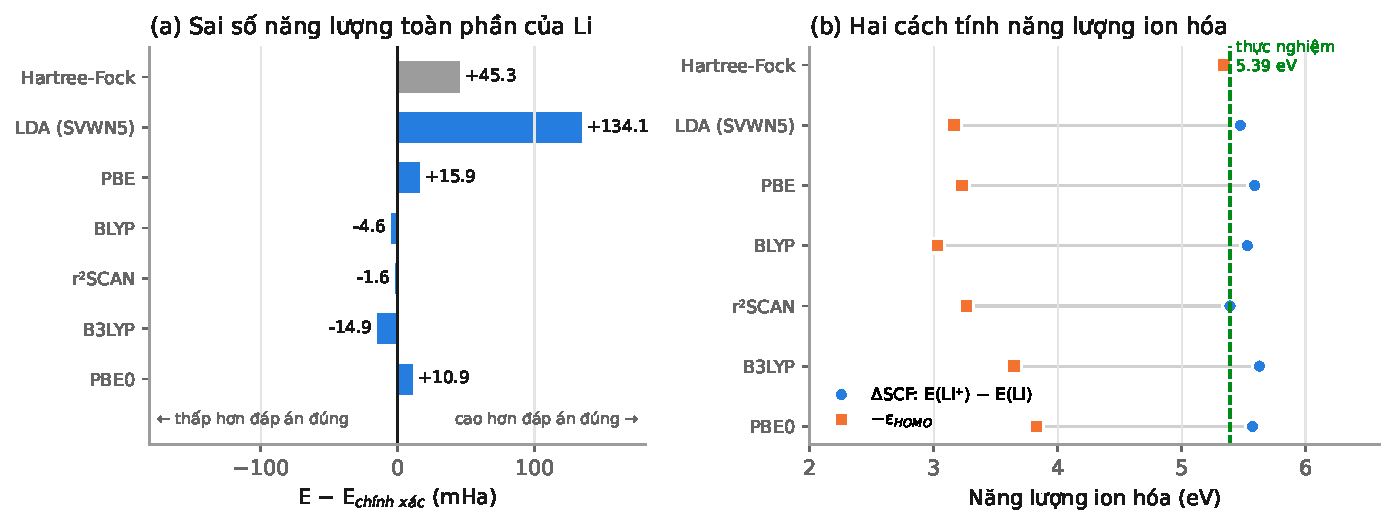
\includegraphics[width=\textwidth]{04_dft_li.pdf}
\caption{(a) Sai số năng lượng toàn phần của Li với từng phiếm hàm (thanh xám: HF). Một số phiếm hàm cho năng lượng \emph{thấp hơn} đáp án đúng. (b) Năng lượng ion hóa tính bằng hiệu năng lượng (tròn xanh) và bằng $-\varepsilon_{\rm HOMO}$ (vuông cam); vạch xanh lá là thực nghiệm. (Script \code{04\_dft.py})}
\label{fig:dftli}
\end{figure}

Bảng~\ref{tab:dft} và hình~\ref{fig:dftli} cho bốn bài học.

\paragraph{1. LDA sai năng lượng toàn phần rất nhiều.} LDA cao hơn đáp án $\ErrLDA\mHa$ (khoảng 3.7\,eV), tệ hơn cả HF. Nguyên tử khác xa một ``khí electron đồng nhất''.

\paragraph{2. DFT xấp xỉ không cho cận trên.} B3LYP cho năng lượng thấp hơn đáp án đúng ($\ErrBthreeLYP\mHa$). Khác với HF hay CI, năng lượng DFT với phiếm hàm xấp xỉ \emph{không} tuân theo nguyên lý biến phân đối với năng lượng thật. ``Thấp hơn'' không có nghĩa ``tốt hơn''.

\paragraph{3. Hiệu năng lượng tốt hơn năng lượng.} Dù LDA sai năng lượng toàn phần tới $\ErrLDA\mHa$, năng lượng ion hóa tính bằng hiệu $E(\text{Li}^+)-E(\text{Li})$ chỉ là $\IEdeltaLDA\eV$, so với thực nghiệm $5.39\eV$. Sai số của Li và Li$^+$ (cùng lõi 1s$^2$) \textbf{triệt tiêu nhau}. Đây là lý do DFT hữu ích trong hóa học: hóa học quan tâm tới \emph{hiệu} năng lượng (năng lượng phản ứng, liên kết), và sai số thường triệt tiêu một phần.

Riêng r$^2$SCAN cho năng lượng ion hóa trùng thực nghiệm tới $0.01\eV$. Đừng vội coi đó là thành công: với Li, các phiếm hàm meta-GGA rất nhạy với lưới tích phân và tập cơ sở, và nghiên cứu chuẩn của Lehtola (2023) thậm chí không đạt được hội tụ SCF cho r$^2$SCAN ở giới hạn tập cơ sở \cite{Lehtola2023}. Sự trùng khớp này nhiều khả năng là ngẫu nhiên.

\paragraph{4. Năng lượng orbital cao nhất sai nặng.} Với phiếm hàm chính xác, $-\varepsilon_{\rm HOMO}$ phải bằng năng lượng ion hóa $5.39\eV$. LDA cho $\HomoLDA\eV$, PBE $\HomoPBE\eV$, B3LYP $\HomoBthreeLYP\eV$: thiếu khoảng 40\%. Trong khi đó HF (định lý Koopmans) cho $\HomoHF\eV$. Thủ phạm là \textbf{lỗi tự tương tác}.

\section{Lỗi tự tương tác}

\begin{eli5}[sợ chính cái bóng của mình]
Một electron đơn lẻ không thể tự đẩy chính mình. Nhưng số hạng Hartree $J[n]$ tính lực đẩy của \emph{toàn bộ} đám mây điện tích lên chính nó, kể cả phần ``electron tự đẩy mình''. Với phiếm hàm chính xác, phần trao đổi xóa sạch sự tự đẩy giả tạo này (như Hartree--Fock làm được, chương~\ref{ch:hf}). Phiếm hàm xấp xỉ chỉ xóa được phần lớn, giống như một người soi gương rồi sợ chính cái bóng của mình.
\end{eli5}

Phép thử sạch nhất là nguyên tử H: chỉ có một electron, không có tương quan, đáp án đúng $E=-0.5\Ha$ và $-\varepsilon_{\rm HOMO}=13.6\eV$. Cột cuối của bảng~\ref{tab:dft} cho thấy LDA sai $\HerrLDA\mHa$, PBE sai $\HerrPBE\mHa$ (gần đúng nhờ may mắn: sai số trao đổi và tương quan gần triệt tiêu nhau), B3LYP sai $\HerrBthreeLYP\mHa$, trong khi HF chỉ sai $\HerrHF\mHa$ (do tập cơ sở). Về năng lượng orbital, $-\varepsilon$ của H theo LDA chỉ khoảng $\HhomoLDA\eV$, theo PBE $\HhomoPBE\eV$, so với $13.6\eV$. Thế trao đổi--tương quan của LDA và GGA tắt quá nhanh khi ra xa (theo hàm mũ thay vì $-1/r$), làm electron ngoài cùng bị ``giữ'' quá lỏng. Đây là gốc rễ của nhiều thất bại khác của DFT: khe năng lượng của chất bán dẫn bị đánh giá thấp, điện tích bị trải quá rộng \cite{Cohen2008}.

\begin{figure}[h]
\centering
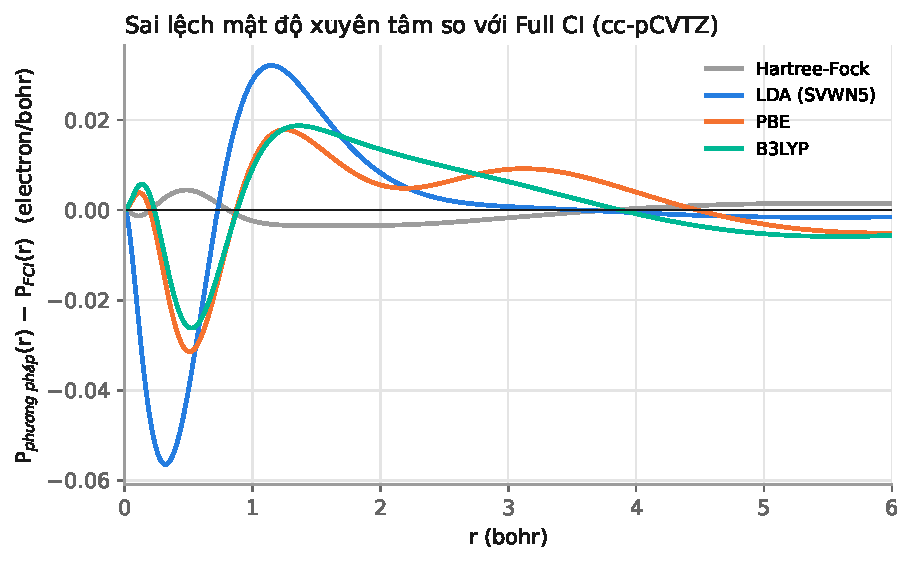
\includegraphics[width=0.8\textwidth]{04_sai_lech_mat_do.pdf}
\caption{Mật độ xuyên tâm của HF, LDA, PBE và B3LYP trừ đi mật độ Full CI (gần như chính xác), cùng tập cơ sở cc-pCVTZ. Cả ba phiếm hàm đều ``rút'' mật độ khỏi đỉnh lớp 1s ($r\approx0.3$--$0.5\bohr$) và dồn ra vùng giữa hai lớp vỏ ($r\approx1$--$2\bohr$), LDA mạnh nhất. Tổng sai lệch $\int|\Delta P|\,dr$ là 0.014 electron cho HF và khoảng 0.06 electron cho cả ba phiếm hàm: với nguyên tử nhỏ này, mật độ HF gần mật độ chính xác hơn mật độ DFT. (Script \code{04\_dft.py})}
\label{fig:matdodft}
\end{figure}

\section{Các thất bại khác đã biết}
\begin{itemize}
\item \textbf{Lực phân tán (van der Waals):} lực hút yếu giữa các phân tử trung hòa đến từ dao động mật độ tương quan ở hai nơi xa nhau. LDA và GGA chỉ ``nhìn'' mật độ tại chỗ nên bỏ sót. Thực tế người ta cộng thêm hiệu chỉnh kiểu DFT-D3 \cite{Grimme2010}.
\item \textbf{Tương quan mạnh:} khi nhiều cấu hình gần suy biến (kéo giãn liên kết, nhiều oxit kim loại chuyển tiếp), một định thức Kohn--Sham với phiếm hàm xấp xỉ thất bại. Đây là bài toán ``ít được giải quyết nhất'' của DFT \cite{Mardirossian2017}.
\item \textbf{Khe năng lượng:} LDA và GGA đánh giá thấp khe năng lượng của chất bán dẫn và cách điện khoảng 40\% \cite{PerdewLevy1983}.
\item \textbf{Không có cách cải thiện có hệ thống:} khác với chuỗi HF $\to$ MP2 $\to$ CCSD $\to$ CCSD(T) $\to$ FCI, không có ``núm vặn'' nào đảm bảo phiếm hàm mới tốt hơn cho mọi hệ. Có hàng trăm phiếm hàm khác nhau.
\end{itemize}

\section{Vì sao DFT vẫn thống trị?}
\begin{itemize}
\item \textbf{Chi phí:} Kohn--Sham với LDA hoặc GGA tăng như $N^3$ theo kích thước hệ, rẻ hơn HF một bậc, và rất rẻ so với CCSD(T) ($N^7$). DFT xử lý được hàng trăm tới hàng nghìn nguyên tử.
\item \textbf{Độ chính xác ``đủ dùng'':} với hiệu năng lượng (phản ứng, cấu trúc, tần số dao động), các hybrid tốt thường sai vài kcal/mol.
\item \textbf{Tầm ảnh hưởng:} theo danh sách 100 bài báo được trích dẫn nhiều nhất mọi thời đại của tạp chí Nature (2014), 12 bài liên quan tới DFT; bài của Lee--Yang--Parr (1988) đứng thứ 7 và bài B3 của Becke (1993) đứng thứ 8 \cite{VanNoorden2014}.
\end{itemize}

\begin{ghinho}
\begin{itemize}
\item DFT thay hàm sóng $3N$ chiều bằng mật độ 3 chiều. Định lý Hohenberg--Kohn đảm bảo mật độ chứa mọi thông tin, nhưng không cho dạng của phiếm hàm.
\item Kohn--Sham dùng một hệ ``diễn viên'' không tương tác có cùng mật độ; mọi phần khó gói vào $E_{xc}$, thứ phải xấp xỉ (LDA, GGA, meta-GGA, hybrid\ldots).
\item Với Li: năng lượng toàn phần có thể sai nhiều (LDA $\ErrLDA\mHa$) và có thể thấp hơn đáp án (B3LYP), nhưng hiệu năng lượng như năng lượng ion hóa thì tốt nhờ triệt tiêu sai số.
\item Lỗi tự tương tác làm $-\varepsilon_{\rm HOMO}$ của LDA/GGA thiếu khoảng 40\% năng lượng ion hóa. Không có cách cải thiện phiếm hàm có hệ thống như chuỗi CC.
\end{itemize}
\end{ghinho}
